\section{Overview of \Treebeard{}}

% \begin{itemize}
%   \item The compiler performs a number of optimizations on the HIR and MIR to improve the performance of the generated code.
%   \item Optimizations in HIR mainly transform the model itself. Tiling, tree reordering and padding are some of the 
%   optimizations that are performed on the HIR. \TODO{Should we use the MICRO paper overview for this part?}
%   \item Explain lowering to MIR using the schedule here.
%   \item Optimizations on the MIR include tree walk unrolling, tree walk interleaving, loop tiling, parallelization etc.
% \end{itemize}

\Treebeard{} takes a serialized decision tree ensemble as input (
XGBoost JSON, ONNX etc.) and automatically generates an optimized inference function
that can either target CPUs or GPUs. 
Figure \ref{Fig:CompilerStructure} shows the structure of the \Treebeard{} compiler. 
The inference computation is lowered through three intermediate representations
-- high-level IR (HIR), mid-level IR (MIR) and low-level IR (LIR). The LIR is
finally lowered to LLVM and then JIT'ed to the specified target processor. 
\Treebeard{} is built using the open-source \TreebeardOLD{} infrastructure~\cite{Treebeard}.
% Since the \TreebeardOLD{} infrastructure was originally designed to target CPUs,
% significant extensions were required to support schedule-guided compilation for CPUs and GPUs. 
The \TreebeardOLD{} infrastructure targets CPUs.
It lacks a scheduling language and does not support generating code for 
different implementation strategies. We enhance \TreebeardOLD{}  
to support schedule-guided compilation for CPUs and GPUs.
The parts \Treebeard{} that are new or significantly different compared to \TreebeardOLD{}
are shown as shaded boxes in Figure \ref{Fig:CompilerStructure}.
% However, it implements several optimizations on the HIR and MIR that 
% can be leveraged across target processors and we find that some these 
% are beneficial for GPUs as well. 
% This reuse of optimizations is possible 
% because the intermediate representations on which these optimizations are performed 
% are abstract and are designed to be target-independent. We briefly review these 
% optimizations below. 

\begin{figure}[htb]
  \centering
  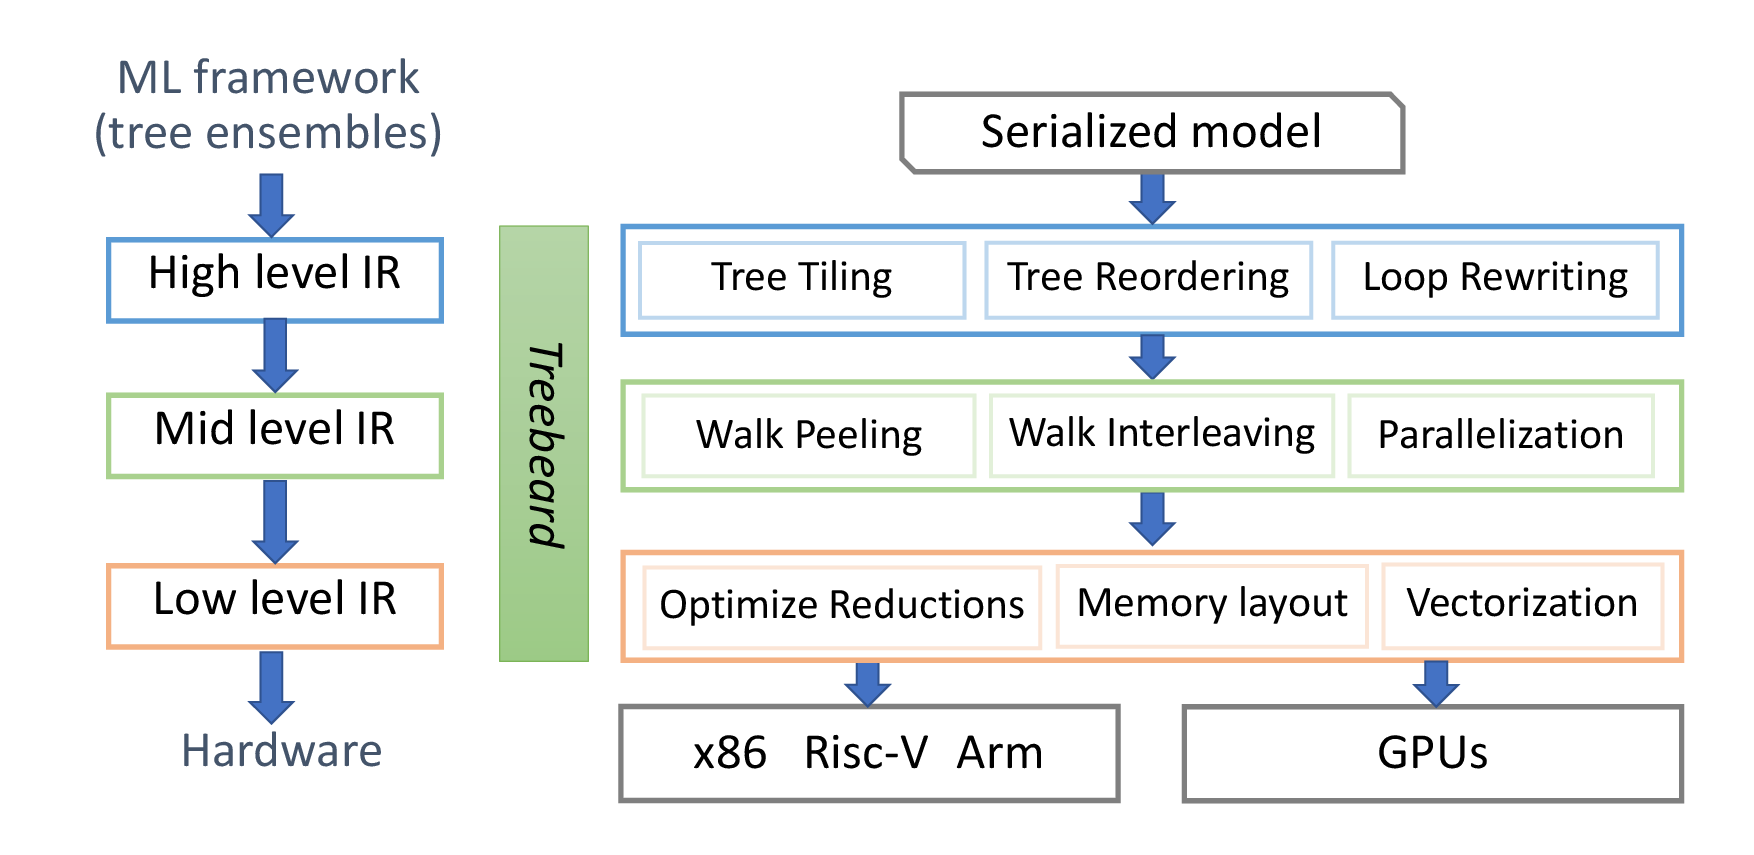
\includegraphics[width=\linewidth]{figures/compiler.png}
  \caption{\Treebeard{} compiler structure.}
  \label{Fig:CompilerStructure}
\end{figure}

Table \ref{Tab:IRSpecification} lists the operations in the three IRs. 
In HIR, the model is represented as a collection of binary trees. This abstraction
allows the implementation of optimizations that require the manipulation of the model
or its constituent trees. We extend the \TreebeardOLD{} infrastructure with loop rewrites on 
the HIR that are implemented through the scheduling language (Section \ref{sec:schedule}).
The \emph{schedule} is implemented as an MLIR attribute on the \op{predictEnsemble} operation.
We use this object to implement the automatic scheduling described in Section \ref{sec:exploring}. 
We reuse HIR transformations to reorder and pad trees from \TreebeardOLD{}.
The tree transformations that reorder and pad trees are used in conjunction 
with loop transformations like splitting to specialize inference code as the example 
in Section \ref{sec:motivation} shows. Also, we enable tree padding only if the schedule 
specifies unrolling of tree walks.
% Figure \ref{Fig:HIRExample} shows this representation for a model 
% with four trees and how the model can be transformed. The model contains two trees of 
% depth 1 and two trees of depth 2 (\circled{A}). The right side of the diagram shows the models after 
% padding and reordering (\circled{B}). Padding makes all leaves in a tree the same depth (Trees 2 and
% 4 are padded). Trees are reordered so that trees of the same depth are together (Trees 
% 2 and 3 are swapped). We use this model as a running example for the rest of the section.
% After these model-level optimizations are performed on the HIR, the 
% code is lowered to the mid-level IR (MIR) as dictated by a  
% \emph{\textbf{schedule}}. The schedule determines how to traverse
% the iteration space that goes over the trees and input rows 
% by specifying how loops are to be tiled, 
% parallelized, mapped to GPU grid and block dimensions etc.
% (Details in Section \ref{sec:schedule}). While MIR is a loop-based IR that 
% explicitly encodes details of the iteration space has to be traversed, 
% it still abstracts details about the in-memory representation of the model. 

The HIR is lowered to MIR as dictated by the \emph{schedule}.
Optimizations like tree-walk unrolling and tree-walk interleaving
are performed on the MIR. 
% These optimizations are beneficial for GPUs as well.
% and the design of \TreebeardOLD{} allows us to reuse the tree-walk 
% unrolling and tree-walk interleaving optimizations on the MIR for GPUs.
% While building \Treebeard{}, we found that
One surprising thing we found while developing \Treebeard{} was that 
we could use ILP to improve performance on GPUs. 
One of the performance bottlenecks in inference code targeted 
to GPUs was that warps spent significant time being stalled. We were able to 
alleviate this bottleneck by interleaving tree walks. 
% This significantly improved performance of generated 
% code. The fact that exploiting ILP improved performance on GPUs was surprising. 

In the generated MIR, the compiler uses the \op{reduce} op from 
the \op{reduction} dialect we design (details in Section \ref{sec:reduction})
to represent reduction operations. The lowering of the \op{reduce} operation 
involves introducing temporary buffers and splitting the operation  
to correctly implement reduction in the presence of 
parallel loops. This process, that we call \textbf{\emph{legalization}}, is 
described in Section \ref{sec:reduction}. 

% \TODO{Should we talk about how interleaving is implemented as a 
% statemachine and therefore it can be used across representations 
% and tile traversal techniques?}

The MIR is further lowered to a low-level IR (LIR). 
Significant changes to \TreebeardOLD{} were required to get
LIR to correctly lower to GPU code. The most important of these was 
changing how the compiler implements support for in-memory 
representations of models (Section \ref{sec:representations}).
% With these design changes, we were able to reuse much of the CPU 
% implementation while customizing some parts for GPUs (for example,
% buffers need to be allocated differently for CPU and GPU, caching 
% is implemented differently etc.). 
Also, when the target processor is a GPU, the required memory transfers and kernel
invocations are inserted into the LIR. Additionally, buffers 
to hold model values are inserted and abstract tree operations are lowered to
explicitly refer to these buffers.
% This lowering is controlled by 
% a plugin mechanism which enables different in-memory representations to 
% be added to the compiler by implementing an interface 
% (Section \ref{sec:representations}). Vectorization of tree traversals
% is also explicitly represented in LIR.
Subsequently, the LIR is lowered to LLVM and then JIT'ed to the 
specified target processor.
% \subsection{Optimizations on High-Level IR}
% We augment the existing \TreebeardOLD{} infrastructure with loop rewrites on 
% the HIR that are implemented through the scheduling language (Section \ref{sec:schedule}).
% We use these to implement the automatic scheduling described in Section \ref{sec:exploring}. 
% Additionally, the \TreebeardOLD{} infrastructure implements HIR transformations to reorder and pad 
% trees. It also implements tree tiling transformations on the HIR \cite{Treebeard}. We reuse the 
% reordering and padding transformations on the HIR for GPUs. However, we found that 
% tiling trees was not beneficial for GPUs. This is because the tiling transformation
% introduces redundant computation inorder to vectorize computation on CPUs where 
% all lanes need to follow the same control flow. However, on SIMT GPUs, we find that 
% the benefits of tiling (coalescing memory accesses) do not outweigh the cost of
% redundant computation. We leave an investigation of this for future work.

% \subsection{Optimizations on Mid-Level IR}
% The original \TreebeardOLD{} infrastructure implements optimizations like 
% tree-walk unrolling, tree-walk interleaving, and parallelization
% on the MIR. These optimizations are beneficial for GPUs as well.
% and the design of \TreebeardOLD{} allows us to reuse the tree-walk 
% unrolling and tree-walk interleaving optimizations on the MIR for GPUs.

% While building \Treebeard{}, we found that one of the performance bottlenecks on the 
% GPU was that warps spent significant time being stalled. Since GPUs 
% implement scoreboarding~\cite{HennesseyPatterson}, we were able to alleviate this bottleneck by
% interleaving tree walks. This significantly improved performance of generated 
% code. We found it surprising that the use of ILP could benefit 
% performance on the GPU.  
% \TODO{Should we talk about how interleaving is implemented as a 
% statemachine and therefore it can be used across representations 
% and tile traversal techniques?}

% \subsection{A Note on Low-level IR}
% Significant changes to the original \TreebeardOLD{} design were required to get
% LIR to correctly lower to GPU code. The most important of these was 
% the change to how the compiler implements support for in-memory 
% representations of models (Section \ref{sec:representations}).
% With these design changes, we were able to reuse much of the CPU 
% implementation while customizing some parts for GPUs (for example,
% buffers need to be allocated differently for CPU and GPU, caching 
% is implemented differently etc.). 